%%%%%%%%%%%%%%%%%%%%%%%%%%%%%%%%%%%%%%%%%%%%%%%%%%%%%%%%%%%%%%%%%%%%%%%%%%%%%%%%
%2345678901234567890123456789012345678901234567890123456789012345678901234567890
%        1         2         3         4         5         6         7         8

\documentclass[letterpaper, 10 pt, conference]{ieeeconf}  % Comment this line out if you need a4paper

%\documentclass[a4paper, 10pt, conference]{ieeeconf}      % Use this line for a4 paper

\IEEEoverridecommandlockouts                              % This command is only needed if 
                                                          % you want to use the \thanks command

\overrideIEEEmargins                                      % Needed to meet printer requirements.

% See the \addtolength command later in the file to balance the column lengths
% on the last page of the document

% The following packages can be found on http:\\www.ctan.org
\usepackage{graphicx} % for pdf, bitmapped graphics files
\usepackage{epstopdf }
%\usepackage{epsfig} % for postscript graphics files
\usepackage{mathptmx} % assumes new font selection scheme installed
\usepackage{times} % assumes new font selection scheme installed
\usepackage{amsmath} % assumes amsmath package installed
\usepackage{amssymb}  % assumes amsmath package installed
\usepackage[hyphens]{url}
\usepackage{nicefrac}
\usepackage{enumerate} % allows enumeration using letters instead of numbers [Added by thomas]
\usepackage{booktabs}  % allows layouting nicer tables [Added by thomas]
\usepackage[loose]{units}
\usepackage{import}
\usepackage{color}
\usepackage{gensymb}
\usepackage{algorithm2e}
\DeclareMathAlphabet{\pazocal}{OMS}{zplm}{m}{n}
\let\oldnl\nl% Store \nl in \oldnl
\newcommand{\nonl}{\renewcommand{\nl}{\let\nl\oldnl}}% Remove line number for one line

\makeatletter
\newcommand{\nosemic}{\renewcommand{\@endalgocfline}{\relax}}% Drop semi-colon ;
\newcommand{\dosemic}{\renewcommand{\@endalgocfline}{\algocf@endline}}% Reinstate semi-colon ;
\newcommand{\pushline}{\Indp}% Indent
\newcommand{\popline}{\Indm\dosemic}% Undent
\makeatother


%#####################################
% lestefan: include pstricks'ed stuff. annoyingly, this will only work on apple. how can we distinguish OS?
\newcommand{\executeiffilenewer}[3]{%
\ifnum\pdfstrcmp{\pdffilemoddate{#1}}%
{\pdffilemoddate{#2}}>0%
{\immediate\write18{#3}}\fi%
}
\newcommand{\includesvg}[1]{%
\IfFileExists{/Applications/Inkscape.app/Contents/Resources/bin/inkscape} % aha, it's an apple
{
\IfFileExists{./images/#1.pdf}{
\executeiffilenewer{./images/#1.svg}{./images/#1.pdf}%
{/Applications/Inkscape.app/Contents/Resources/bin/inkscape -z -D --file=./images/#1.svg %
--export-pdf=./images/#1.pdf --export-latex}%
}  
{
\immediate\write18{/Applications/Inkscape.app/Contents/Resources/bin/inkscape -z -D --file=./images/#1.svg %
--export-pdf=./images/#1.pdf --export-latex}
}
}
{
%else:
\IfFileExists{./images/#1.pdf}{
\executeiffilenewer{./images/#1.svg}{./images/#1.pdf}%
{inkscape -z -D --file=./images/#1.svg %
--export-pdf=./images/#1.pdf --export-latex}%
}
}
{
\immediate\write18{inkscape -z -D --file=./images/#1.svg %
--export-pdf=./images/#1.pdf --export-latex}
}
\import{./images/}{#1.pdf_tex}%
}
%#####################################


\title{\LARGE \bf A solar-powered hand-launchable UAV for low-altitude multi-day continuous flight}

\author{Philipp Oettershagen$^{1}$, Amir Melzer, Thomas Mantel, Konrad Rudin, \\ Rainer Lotz, Dieter Siebenmann, Stefan Leutenegger, Kostas Alexis and Roland Siegwart% <-this % stops a space
\thanks{All authors are part of the Autonomous Systems Lab, Swiss Federal Institute of Technology Zurich (ETH Zurich). Leonhardstrasse 21, 8092 Zurich, Switzerland. }
\thanks{$^{1}$ E-Mail:{\tt philipp.oettershagen@mavt.ethz.ch}}%
\thanks{*This work was supported by the EU-FP7 research projects ICARUS and SHERPA as well as a number of project partners and generous individuals, see http://www.atlantiksolar.ethz.ch/  }% <-this % stops a space
 }

\begin{document}

\maketitle
\thispagestyle{empty}
\pagestyle{empty}

%%%%%%%%%%%%%%%%%%%%%%%%%%%%%%%%%%%%%%%%%%%%%%%%%%%%%%%%%%%%%%%%%%%%%%%%%%%%%%%%
\begin{abstract}
%%%%%%%%%%%%%%%%%%%%%%%%%%%%%%%%%%%%%%%%%%%%%%%%%%%%%%%%%%%%%%%%%%%%%%%%%%%%%%%%
This paper presents the conceptual design, detailed development and flight testing of \textit{AtlantikSolar}, a 5.6m-wingspan solar-powered Low-Altitude Long-Endurance (LALE) Unmanned Aerial Vehicle (UAV) designed and built at ETH Zurich. The UAV is required to provide perpetual endurance at a geographic latitude of 45\degree N in a 4-month window around June 21\textsuperscript{st}. A improved conceptual design method is used maximizing perpetual flight robustness with respect to local meteorological disturbances such as clouds or winds. Airframe, avionics hardware, state estimation and control method development for autonomous flight operations are described. Flight test results include a 12-hour flight relying solely on batteries to replicate night-flight conditions. In addition we present flight results from Search-And-Rescue field trials where a camera and processing pod was mounted on the aircraft to create high-fidelity 3D-maps of a simulated disaster area. 
\end{abstract}

%%%%%%%%%%%%%%%%%%%%%%%%%%%%%%%%%%%%%%%%%%%%%%%%%%%%%%%%%%%%%%%%%%%%%%%%%%%%%%%
% SECTION1: INTRODUCTION
%%%%%%%%%%%%%%%%%%%%%%%%%%%%%%%%%%%%%%%%%%%%%%%%%%%%%%%%%%%%%%%%%%%%%%%%%%%%%%%
%%%%%%%%%%%%%%%%%%%%%%%%%%%%%%%%%%%%%%%%%%%%%%%%%%%%%%%%%%%%%%%%%%%%%%%%%%%%%%%
\section{INTRODUCTION}
%%%%%%%%%%%%%%%%%%%%%%%%%%%%%%%%%%%%%%%%%%%%%%%%%%%%%%%%%%%%%%%%%%%%%%%%%%%%%%%

%%%%%%%%%%%%%%%%%%%%%%%%%%%%%%%%%%%%%%%%%%%%%%%%%%%%%%%%%%%%%%%%%%%%%%%%%%%%%%%
%\subsection{Solar-powered UAVs for perpetual flight endurance}
%%%%%%%%%%%%%%%%%%%%%%%%%%%%%%%%%%%%%%%%%%%%%%%%%%%%%%%%%%%%%%%%%%%%%%%%%%%%%%%

When carefully designed, solar-electrically powered fixed-wing Unmanned Aerial Vehicles (UAVs) exhibit significantly increased flight endurance over purely-electrically or even gas-powered aerial vehicles. Given certain environmental conditions, a solar-powered UAV creates surplus energy when observed over a full day-night cycle, i.e. it will fully recharge its batteries during the day to continue flight through the night and potentially subsequent day-night cycles. Long endurance - and especially this multi-day continuous flight capability termed \emph{perpetual endurance} - is of significant interest for large-scale mapping, observation or telecommunications relay applications as they occur in Search-And-Rescue (SAR) missions, industrial or agricultural inspection, meteorological surveys, border patrol and more~\cite{NASA_Pathfinder}.

Recently, interest in employing solar-powered large-scale (wingspan above 20m) High-Altitude Long-Endurance (HALE) UAVs as \emph{atmospheric satellites} - i.e. stationary/loitering platforms e.g. for telecommunications relay - has peaked. Notable examples of this trend are \textit{Solara}~\cite{IEEE_AtmosphericSatellites} and \textit{Zephyr}, the latter of which has already demonstrated a continuous flight of 14 days~\cite{QinetiQ_Zephyr14dayRecord}. In contrast, smaller scale solar-powered UAVs are mostly designed for Low-Altitude Long Endurance (LALE) applications. While they have to cope with the more challenging meteorological phenomena of the lower atmosphere (clouds, rain, wind gusts or thermals), they generally have the advantage of providing less cloud-obstructed and higher-resolution imaging capability, lower complexity and cost as well as easier and faster handling (e.g. through hand-launchability) as beneficial in First-Aid SAR scenarios. Research in small-scale solar UAVs targeting perpetual endurance has been relatively sparse, with most research including~\cite{Morton_ICRA2013} focussing on conceptual design studies without extensive flight experience. However, Cocconi's \textit{SoLong}~\cite{Cocconi_SoLong} performed a continuous 48-hour flight using solar power and thermal updraft hunting in 2005, though with limited airplane autonomy. Noth presents the conceptual design methods, realization and experimental flight results of the 3.2m wing span \textit{SkySailor}~\cite{Noth_PhD}, which demonstrated a 27-hour solar-powered continuous flight without the use of thermals in 2008. 

\begin{figure}[b]
    \centering
    \includegraphics[width=.98\linewidth]{images/atlantiksoar_figure_v3_vSmall}
    \caption{The AtlantikSolar solar-powered UAV developed at ETH Zurich}
    \label{fig:AtlantikSolarCollage}
\end{figure}

%%%%%%%%%%%%%%%%%%%%%%%%%%%%%%%%%%%%%%%%%%%%%%%%%%%%%%%%%%%%%%%%%%%%%%%%%%%%%%%
%\subsection{Contributions of this paper}
%%%%%%%%%%%%%%%%%%%%%%%%%%%%%%%%%%%%%%%%%%%%%%%%%%%%%%%%%%%%%%%%%%%%%%%%%%%%%%%

This paper aims to extend the work of \cite{Cocconi_SoLong,Noth_PhD} by presenting \textit{AtlantikSolar}, a solar-powered LALE-UAV with a wingspan of 5.6m designed towards more robust multi-day autonomous operation capabilities while providing the option to use an advanced optical and infrared sensor system together with on-board computation resources developed at ETH Zurich. The contribution of the paper lies in presenting the complete development cycle from conceptual UAV design to actual testing and missions, or more specifically
  
 \begin{enumerate}
\item the application and extension of the conceptual design approach in \cite{Noth_PhD,Leutenegger_JIRS} towards more robust multi-day flight under sub-optimal meteorological conditions, 
\item the realization of the conceptual design in UAV hardware, i.e. structure, low-level electronics \& avionics, 
\item the development of on--board state estimation algorithms and flight control methods based on an \textit{Extended Kalman Filter} (EKF) and PID control with non-linear guidance and
\item the discussion of flight test results including long-endurance flight (up to 12h) and mapping results during exemplary SAR missions.
\end{enumerate}

%+ picture of AtlantikSolar in flight
%1) Kostas from side
%2) ``Aerobatic picture'' from TJ
%3) Maybe landing picture.
%- Make sure to include some with sensor pod

%%%%%%%%%%%%%%%%%%%%%%%%%%%%%%%%%%%%%%%%%%%%%%%%%%%%%%%%%%%%%%%%%%%%%%%%%%%%%%%
% SECTION2: CONCEPTUAL DESIGN
%%%%%%%%%%%%%%%%%%%%%%%%%%%%%%%%%%%%%%%%%%%%%%%%%%%%%%%%%%%%%%%%%%%%%%%%%%%%%%%
%%%%%%%%%%%%%%%%%%%%%%%%%%%%%%%%%%%%%%%%%%%%%%%%%%%%%%%%%%%%%%%%%%%%%%%%%%%%%%%
\section{CONCEPTUAL DESIGN}
%%%%%%%%%%%%%%%%%%%%%%%%%%%%%%%%%%%%%%%%%%%%%%%%%%%%%%%%%%%%%%%%%%%%%%%%%%%%%%%

%%%%%%%%%%%%%%%%%%%%%%%%%%%%%%%%%%%%%%%%%%%%%%%%%%%%%%%%%%%%%%%%%%%%%%%%%%%%%%%
\subsection{Methodology} \label{sec:ConceptualDesignMethodology}
%%%%%%%%%%%%%%%%%%%%%%%%%%%%%%%%%%%%%%%%%%%%%%%%%%%%%%%%%%%%%%%%%%%%%%%%%%%%%%%

The conceptual design methodology for solar-powered UAVs used in this paper was developed at ETH Zurich by \cite{Noth_PhD,Leutenegger_JIRS} and is briefly summarized below. To analyze flight performance and a potential perpetual flight capability, the energy input/output-balance needs to be modeled. The total required nominal electrical output power
\begin{equation} \label{eqn:P_out}
P_{out}^{\,nom}=\frac{P_{level}}{\eta_{prop}}+P_{av}+P_{pld}
\end{equation}
consists of the required electrical propulsion power for level-flight $\frac{P_{level}}{\eta_{prop}}$ , where $\eta_{prop}$ includes propeller, gearbox, motor, and motor-controller efficiency, and the necessary avionics and payload power $P_{av}$ and $P_{pld}$. The aircraft is assumed to fly at the airspeed of minimum aerodynamic level-flight power
\begin{equation} \label{eqn:P_level}
P_{level}=\left(\frac{C_D}{C_L^\frac{3}{2}}\right)_{min}\sqrt{\frac{2(m_{tot}g)^3}{\rho(h)A_{wing}}} .
\end{equation}
Here, $m_{tot}=m_{bat}+m_{struct}+m_{prop}+m_{sm}+m_{av}+m_{pld}$ is the total airplane mass, where structure, propulsion and solar module masses $m_{struct},m_{prop},m_{sm}$ are automatically sized according to \cite{Noth_PhD,Leutenegger_JIRS} and $m_{av},m_{pld}$ are given in table \ref{tab:ConceptDesignParameters}. The local earth gravity is designated by $g$, $A_{wing}$ is the wing area, and $rho$ is air density. The airplane lift and drag coefficients $C_L$ and $C_D$ are retrieved from 2-D airfoil simulations using XFoil \cite{Drela_XFoil}, with $C_D$ being combined with parasitic drag from the airplane fuselage and stabilizers and the induced drag  
\begin{equation} \label{eqn:C_D}
C_{D,ind}=\frac{c_L^2}{\pi\cdot e_0\cdot\lambda} .
\end{equation}
Here, $e_0\approx0.92$ is the Oswald efficiency and $\lambda$ the wing aspect ratio. On the input side, the nominal solar input power
\begin{equation} \label{eqn:P_solar}
P_{solar}^{\,nom}=I\cdot A_{sm}\cdot\eta_{sm}\cdot\eta_{mppt}
\end{equation}
considers the solar module area $A_{sm}=f_{sm}\cdot A_{wing}$ with relative fill-factor $f_{sm}$, module efficiency $\eta_{sm}$, and Maximum Power Point Tracker (MPPT) efficiency $\eta_{mppt}$. The solar radiation $I=I(\varphi,h,t)$ is assumed to be a function of the geographical latitude $\varphi$, the altitude $h$, and the current date and local time $t$, and is modeled as in \cite{Duffie_SolarEngineering}.
The state equation can now be formulated in a simplified form as
\begin{equation}\label{eqn:StateEquations}
\begin{array}{r@{}l}
\frac{dE_{bat}}{dt}&=P_{solar}(\varphi,h,t)-u-P_{av}-P_{pld},\\
\frac{dh}{dt}&=\frac{\eta_{prop}\cdot u-P_{level}(h)}{m_{tot}g} .
\end{array}
\end{equation}
Here, $u$ is the actual electrical power sent to the propulsion system. Simple forward integration of the state equation (\ref{eqn:StateEquations}) gives the battery state of charge (SoC) over time and thus determines the perpetual flight capability.

For the design optimization, we assume that a solar-powered UAV configuration is designed for missions at and around a specific date of the year (DoY) and geographical latitude $\varphi$, and thus $\varphi$ and $DoY$ are fixed parameters. The three design parameters to be optimized are
\begin{itemize}
\item The wingspan $b$ and wing aspect ratio $\lambda$, which specify wing geometry and thus influence the level-power in (\ref{eqn:P_level}) and the solar input power in (\ref{eqn:P_solar}).
\item The battery mass $m_{bat}$ contained in $m_{tot}$ in (\ref{eqn:P_level}) 
\end{itemize}

%%%%%%%%%%%%%%%%%%%%%%%%%%%%%%%%%%%%%%%%%%%%%%%%%%%%%%%%%%%%%%%%%%%%%%%%%%%%%%%
\subsection{Extension of conceptual design optimization criteria}
%%%%%%%%%%%%%%%%%%%%%%%%%%%%%%%%%%%%%%%%%%%%%%%%%%%%%%%%%%%%%%%%%%%%%%%%%%%%%%%

\label{sec:ExtensionOptCriteria}
The conceptual design tool developed in \cite{Noth_PhD,Leutenegger_JIRS} has been extended in two ways: First, it now provides the capability to perform energetic simulations of multi-day solar-powered flight, whereas before only one day-night cycle was considered. Fig. \ref{fig:EnergySimulation} shows the results for incoming solar power $P_{solar}$, required power $P_{out}$, and remaining battery charge $E_{bat}$ obtained for a two day/night cycle flight. Clearly, the initial charge condition $E_{bat}$ at time of sunrise $t_{sr}=min(t(P_{solar}>0))$ for the second day is different than on the first day, which significantly reduces the required charge time until $E_{bat}=E_{bat}^{\,max}$ and leads to increased charge margins with respect to the pure one day/night-cycle simulation. %is this paragraph really needed?
\begin{figure}[tb]
    \centering
    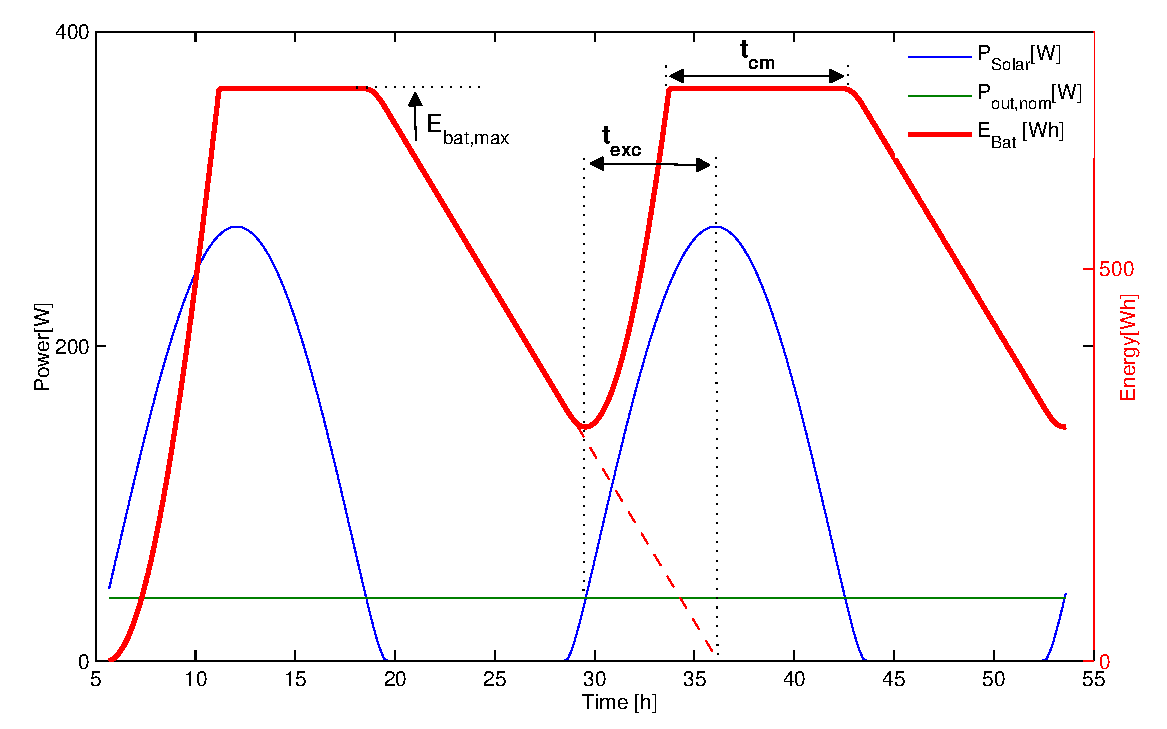
\includegraphics[width=\linewidth]{images/2_EnergySimulation}
    \caption{Energetic simulation of the AtlantikSolar UAV configuration ($b=5.6m$, $\lambda=18.5$, $m_{bat}=3.5kg$), showing input and output power, battery capacity, and performance metrics excess time $t_{exc}$ and charge margin $t_{cm}$ during a 2-day flight.}
    \label{fig:EnergySimulation}
\end{figure}
Second, and more importantly, the optimization criteria are extended with respect to \cite{Noth_PhD,Leutenegger_JIRS} to achieve more robust multi-day flight. In general, a necessary and sufficient condition for perpetual flight is that the excess time $t_{exc}>0$, where 
\begin{equation} \label{eqn:t_exc}
t_{exc}=\frac{E_{bat}(t=t_{eq})}{P_{out}^{\,nom}} \Big| P_{solar}(t>t_{sr})=0
\end{equation}
with ``power-equality time'' $t_{eq}=t(P_{solar}^{\,nom}=P_{out}^{\,nom})$ in the morning. This means that at $t=t_{eq}$ there has to exist remaining battery capacity to continue flight e.g. in case of cloud coverage in the morning. This is why\cite{Noth_PhD,Leutenegger_JIRS} focus on maximizing $t_{exc}$. However, a large $t_{exc}$ does not provide direct robustness against disturbances in $P_{solar}$ during the charging process(e.g. due to clouds). In contrast, when optimizing purely for $t_{exc}$, the methodology in Sec. \ref{sec:ConceptualDesignMethodology} will select the largest battery size (due to the scaling of $P_{level}$ with $m_{bat}$ ) which can still be fully charged unter optimal conditions, but every reduction in $P_{solar}$ will directly decrease $t_{exc}$ due to only partially charged batteries. We thus introduce the charge margin $t_{cm}$ as the time margin between achieving the full charge $E_{bat}=E_{bat}^{\,max}$ and restart of the discharge in the evening. In case of decreased solar power income, $t_{cm}>0$ will provide an additional margin before a decrease in excess time occurs.

The overall approach for increasing robustness with respect to local disturbances in the power income and output is thus to determine the lowest acceptable $t_{exc}$ satisfying the UAV application requirements, and to then optimize the configuration for $t_{cm}$. The exact procedure applied here is:
\begin{enumerate}
\item Choose the nominal operating latitude $\varphi$ and Day-of-Operation $DoY^{nom}$, and the outermost days where perpetual UAV endurance is required $DoY^{min,max}$
\item Obtain $t_{night}^{\,min}$ and $t_{night}^{\,max}$ for the range of $DoY=[DoY^{min},DoY^{max}]$ from \cite{Duffie_SolarEngineering}. 
\item The required excess time $t_{exc,req}$ is now the sum of 
\begin{itemize}
	\item $t_{exc,DoY} = t_{night}^{\,max}-t_{night}^{\,min}$
	\item $t_{exc,clouds}$, to allow a margin for clouds in the morning or evening
	\item $t_{exc,P_{level}}$, to allow a margin for increased power consumption e.g. caused by downdrafts or uncertainties in estimating $P_{level}$
\end{itemize}
\item Perform the design analysis given the methodology in sec. \ref{sec:ConceptualDesignMethodology} for $DoY(t_{night}=t_{night}^{\,min})$. Pre-select the subset $\mathcal{S}$ of configurations satisfying $t_{exc}>t_{exc,req}$.
\item Within $\mathcal{S}$, allow for a set of intermediate configurations $\mathcal{S}_i$ to take into account UAV-specific constraints on $b$, $\lambda$, or $m_{bat}$. Then choose the final configuration $\mathcal{S}_f$  from $\mathcal{S}_i$ to obtain the largest charge margin $t_{cm}$.
\end{enumerate}

This conceptual design methodology is applied below. An alternative conceptual design approach utilizing a weighed version of $t_{exc}$ and $t_{cm}$ is proposed in \cite{Morton_ICRA2013}. 

% less predictable phenomenas such as clouds or winds. 
% local detoriation in the meteorological conditions. 
% AtlantikSolar charge curve is shown in figure above
% Explain(a simplified) POutput and PInput distrubance on this graphic. Name them (a) nominal (b) distrubed POutput (c) disturbed PInput. ???
% We need a mixture of both t_exc and t_cm, and how much we want to optimize exactly w.r.t the two depends on our confidence in the underlying performances. Power consumptino can be tested quite well, but meteo-conditions can not -> t\_cm very important, because t\_exc will then stay the same. If t\_cm is zero, no margin against bad meteo conditions. t\_exc should however still be on the order of some hours( we select t\_exc>~3hours), because this is how long clouds in morning/evening could/might cause P\_Solar~0. Also, minSoC>0.1, as this is limit for Go-Around-Operations.
% - optimizing only towards t\_exc will cause the method to select largest E\_bat which still results in full charge under the specific conditions
 
%%%%%%%%%%%%%%%%%%%%%%%%%%%%%%%%%%%%%%%%%%%%%%%%%%%%%%%%%%%%%%%%%%%%%%%%%%%%%%%
\subsection{Application of Conceptual Design methodology} \label{sec:ConceptDesignApplication}
%%%%%%%%%%%%%%%%%%%%%%%%%%%%%%%%%%%%%%%%%%%%%%%%%%%%%%%%%%%%%%%%%%%%%%%%%%%%%%%

AtlantikSolar operate at a nominal latitude of $\varphi=45°N$ and shall provide perpetual endurance within a +/-2 month window around $DoY_{nom}$=June 21\textsuperscript{st} (April 21\textsuperscript{st}-August 21\textsuperscript{st}). From \cite{Duffie_SolarEngineering}, we find $t_{night}^{\,min}=8.7h$ (June 21\textsuperscript{st}), $t_{night}^{\,max}=10.5h$(April 21\textsuperscript{st}), and thus $t_{exc,DoY}=1.80h$. We choose $t_{exc,clouds}=3.0h$ to account for three hours of full cloud coverage either on the evening or the morning and choose $t_{exc,P_{level}}=0.2\cdot t_{night,max}=2.1h$ to cover increased power consumption due to modelling errors, downdrafts or headwinds. Using $t_{exc,req}=t_{exc,DoY}+t_{exc,clouds}+t_{exc,P_{level}}$, we retrieve $t_{exc,req}=6.9h$ as the minimum required excess time for robust perpetual-flight at the given dates and locations. 

The design methodology tool of section \ref{sec:ConceptualDesignMethodology} is now applied assuming the fixed component performance parameters in Tab. \ref{tab:ConceptDesignParameters}. Fig. \ref{fig:ExcessTimeChargeMargin} shows the resulting plot for $t_{exc}$ versus the optimization variables $b$, $m_{bat}$ and $\lambda=18.5$. The subset $\mathcal{S}$ of configurations satisfying $t_{exc}>t_{exc,req}$ is the region within the blue contour-line. The optimum clearly occurs at large wing spans, however, considering an external size constraint (each of the three wing pieces of AtlantikSolar shall be $<2m$ in wing span to allow proper handling and transport), we choose $b=5.6m$.  The aspect ratio $\lambda=18.5$ is found to provide an optimum in $t_{exc}$ and also allows to seamlessly integrate the solar cells (see Sec. \ref{secsec:Airframe and hardware}) inside the wing chord. The last design choice is now $m_{bat}$, for which we seek to optimize $t_{cm}$ within the previously selected set $\mathcal{S}_i=(\mathcal{S}|b=5.6m, \lambda=18.5)$. As visible in Fig. \ref{fig:ExcessTimeChargeMargin}, $m_{bat}=3.0...7.5kg$ lie within $\mathcal{S}_i$. We choose $m_{bat}=3.5kg$ to optimize $t_{cm}$ and due to practical battery sizing constraints described in Sec. \ref{secsec:Airframe and hardware}. The selected final configuration $\mathcal{S}_f=(\mathcal{S}|m_{bat}=3.5kg, b=5.6m, \lambda=18.5)$ has an overall estimated mass of $m_{tot}=7.22kg$ and yields a predicted $t_{exc}=7.89h$ and $t_{cm}=8.38h$ for the nominal operating date and latitude.
\begin{figure}[tb]
    \centering
    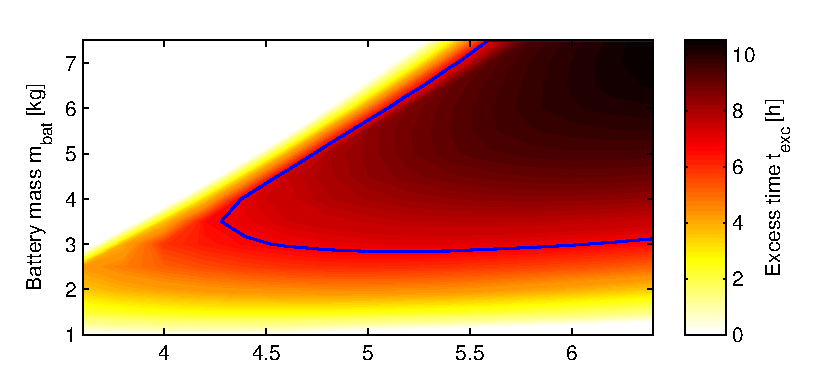
\includegraphics[width=\linewidth]{images/3_excesstime}
    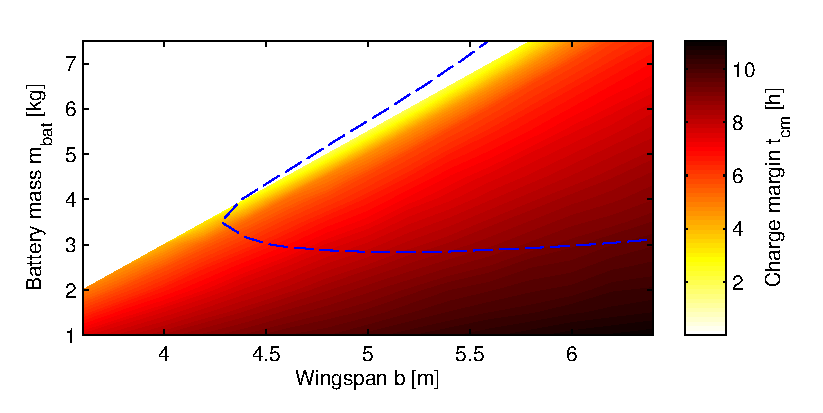
\includegraphics[width=\linewidth]{images/4_chargemargin}
    \caption{Excess time $t_{exc}$ (top) and charge margin $t_{cm}$ (bottom) vs. optimization parameters $b$ and $m_{bat}$, all at $\lambda=18.5$. The configuration subset $\mathcal{S}$ satisfying $t_{exc}>t_{exc,req}$ under our design requirements lies inside the blue contour line.}
    \label{fig:ExcessTimeChargeMargin}
\end{figure}
\begin{table}[h] 
\caption{Fixed parameters for the conceptual design}
\label{tab:ConceptDesignParameters}
\begin{center}
\begin{tabular}{l l l}
\hline Parameter & Value & Description\\ 
\hline $eta_{sm}$ & 0.20&Solar module efficiency\\
\hline $eta_{MPPT}$ & 0.97&MPPT efficiency\\
\hline $eta_{prop}$ & 0.58 &Propulsion system effiency\\
\hline $e_{bat}$ & 874800\unitfrac{J}{kg}&Battery specific energy\\
\hline $f_{sm}$ & 0.94&Solar module fill factor\\
\hline $k_{sm}$ & 0.59$\unitfrac{kg}{m²}$ & Solar module areal density\\
\hline $m_{av}$ & 0.6kg&Avionics mass (including all cabling)\\
\hline $m_{pld}$ & 0.1kg&Payload mass\\
\hline $P_{av}$ & 4.5\unit{W}&Avionics power consumption\\
\hline $P_{pld}$ & 0.0\unit{W}&Payload power consumption\\
\end{tabular}
\end{center}
\end{table}

%%%%%%%%%%%%%%%%%%%%%%%%%%%%%%%%%%%%%%%%%%%%%%%%%%%%%%%%%%%%%%%%%%%%%%%%%%%%%%%
\subsection{Robustness analysis}
%%%%%%%%%%%%%%%%%%%%%%%%%%%%%%%%%%%%%%%%%%%%%%%%%%%%%%%%%%%%%%%%%%%%%%%%%%%%%%%

To verify the multi-day flight robustness of the developed UAV configuration $\mathcal{S}_f$, we analyze its performance considering a set of local disturbances in UAV power input and output, namely
\begin{itemize}
\item The disturbed solar power income $P_{solar}^{\,dist}$, as caused by clouds or fog. Lacking knowledge of the exact spatial and temporal disturbance distribution, we assume the simple scaling
\begin{equation}
P_{solar}^{\,dist}(t) = P_{solar}^{\,nom}(t) \cdot k_{CCF}.
\end{equation}
Here, $k_{CCF}=[0,1]$  represents the current cloud cover factor \cite{Kimura_SolarRadAndClouds}, i.e. the clearness of the atmosphere.
\item The disturbed electrical power output $P_{out}^{\,dist}$. Wind downdrafts, head wind, or gusts may require increased propulsion or actuation power. Again, we assume 
\begin{equation}
P_{out}^{\,dist}(t) = P_{out}^{\,nom}(t) \cdot k_{OPF},
\end{equation}
with $k_{OPF}$ representing the Output Power Factor.
\end{itemize}
\begin{figure}
    \centering
    \includegraphics[width=\linewidth]{images/5_texcRobustness}
    \caption{Excess time $t_{exc}$ under disturbed power input and output for the developed $b=5.6m$, $\lambda=18.5$ configuration: a) $m_{bat}$=3.5kg on June 21\textsuperscript{st} b) $m_{bat}=6.0kg$ on June 21\textsuperscript{st} c) $m_{bat}$=3.5kg on April 21\textsuperscript{st} d) $m_{bat}=6.0kg$ on April 21\textsuperscript{st} }
    \label{fig:ExcessTimeRobustness}
\end{figure}
Fig. \ref{fig:ExcessTimeRobustness} shows the remaining excess time with respect to these disturbances. The UAV configuration developed in section \ref{sec:ConceptDesignApplication} (with $m_{bat}=3.5kg$) still provides perpetual endurance with less than 50\% of the solar power income or if more than 60\% surplus power are required e.g. to compensate for downdrafts on June 21\textsuperscript{st} (Fig.\ref{fig:ExcessTimeRobustness}a). In contrast, a configuation purely optimized towards excess time with $m_{bat}=6.0kg$ (Fig.\ref{fig:ExcessTimeRobustness}b) will yield a higher maximum $t_{exc}$ of 9.5h, however, the robustness with respect to clouds or higher required level power is greatly decreased. On April  21\textsuperscript{st}, the UAV configuration of section \ref{sec:ConceptDesignApplication} still provides solid robustness (Fig.\ref{fig:ExcessTimeRobustness}c), which verifies the $DoY^{\,nom}\pm$ 2 months perpetual endurance requirement. In contrast, the $m_{bat}=6.0kg$ configuration (Fig.\ref{fig:ExcessTimeRobustness}d) can not provide reliable perpetual endurance anymore. Overall, the configuration developed using the extended optimization criteria from Sec. \ref{sec:ExtensionOptCriteria} thus shows significantly improved multi-day flight robustness in comparison with configurations that are purely optimized for maximum excess time.

%%%%%%%%%%%%%%%%%%%%%%%%%%%%%%%%%%%%%%%%%%%%%%%%%%%%%%%%%%%%%%%%%%%%%%%%%%%%%%%
% SECTION3: DETAILED DESIGN AND REALIZATION
%%%%%%%%%%%%%%%%%%%%%%%%%%%%%%%%%%%%%%%%%%%%%%%%%%%%%%%%%%%%%%%%%%%%%%%%%%%%%%%
\section{DETAILED DESIGN AND REALIZATION}

AtlantikSolar (Figs. \ref{fig:AtlantikSolarCollage} and \ref{fig:CAD_AtlantikSolarFull}) is a solar-powered Low-Altitude Long-Endurance(LALE) Unmanned Aerial Vehicle designed for perpetual flight at $\varphi=45°$ geographical latitude from April 21\textsuperscript{st} to August 21\textsuperscript{st}. It was designed and built at ETH Zurich as a lightweight high aspect ratio airplane to achieve minimum sink rate. Although its design is mostly dictated by the requirement for low power consumption, it does provide the option to use visual\&infrared sensor systems and on-board computation ressources in an autonomous operation mode for use in search and rescue or industrial inspection applications. The airplane design is summarized in table \ref{tab:DetailedDesignParameters}. Figure \ref{fig:AtlantikSolar_SystemOverview} presents an overview over the aircraft components topology.

\begin{figure}[tb]
    \centering
    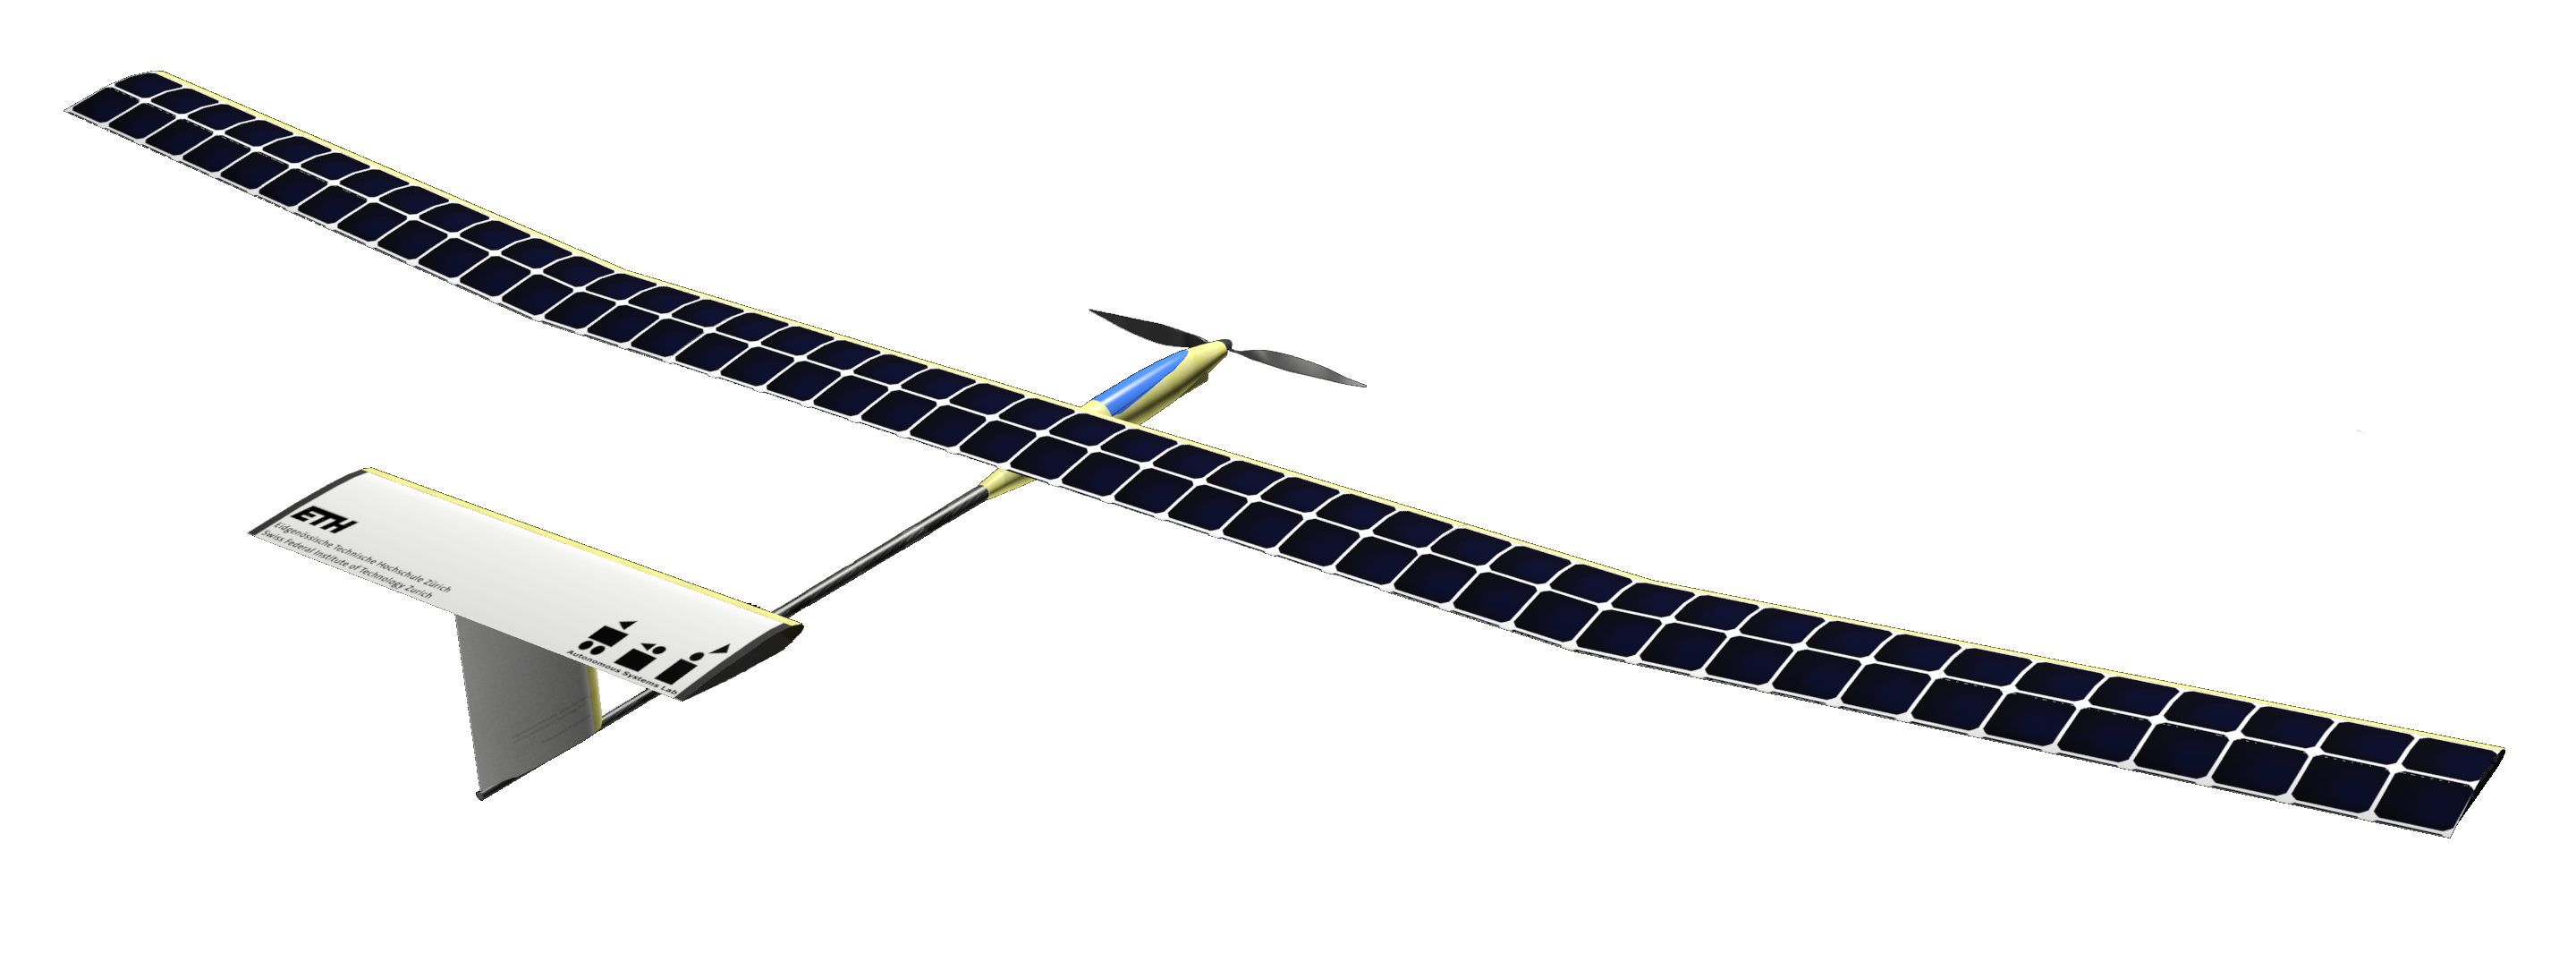
\includegraphics[width=\linewidth]{images/6_CAD_AtlantikSolarFull}
    \caption{The AtlantikSolar UAV features a conventional T-tail configuration with 1 motor, two ailerons, an all-moving elevator and a rudder for actuation.}
    \label{fig:CAD_AtlantikSolarFull}
\end{figure}

\begin{table}
\label{tab:DetailedDesignParameters}
\caption{AtlantikSolar design characteristics}
\begin{center}
\begin{tabular}{l l}
Wing span & 5.65$\unit{m}$\\
\hline Wing chord& 0.305$\unit{m}$\\
\hline Length& \\
\hline Height&\\
\hline Mass& 7.36$\unit{kg}$\\
\hline Battery mass& 3.52$\unit{kg}$\\
\hline Wing loading&4.28$\unitfrac{kg}{m^2}$\\
\hline Stall speed& 8.1$\unitfrac{m}{s}$ TBD\\
\end{tabular}
\end{center}
\end{table}

\subsection{UAV Platform Design}
\subsubsection{Airframe and hardware}

The structure of AtlantikSolar is built in a traditional rib-spar construction method. The wing (Fig. \ref{fig:CAD_AtlantikSolarStructure}) consists of an inner cylindrical carbon-fibre spar to resist torsional wing loads. Four carbon-fibre belts of trapezoidal and laterally-varying cross-section are located around the spar to optimally resist bending loads and to provide maximum wing stiffness to protect the solar cells on the wings. Equally-spaced balsa-wood ribs and the kevlar-reinforced wing leading edge provide structural support for the non-load-carrying outer wing surface. The horizontal and vertical tail planes are constructed in a similar fashion.

\begin{figure}[tb]
    \centering
    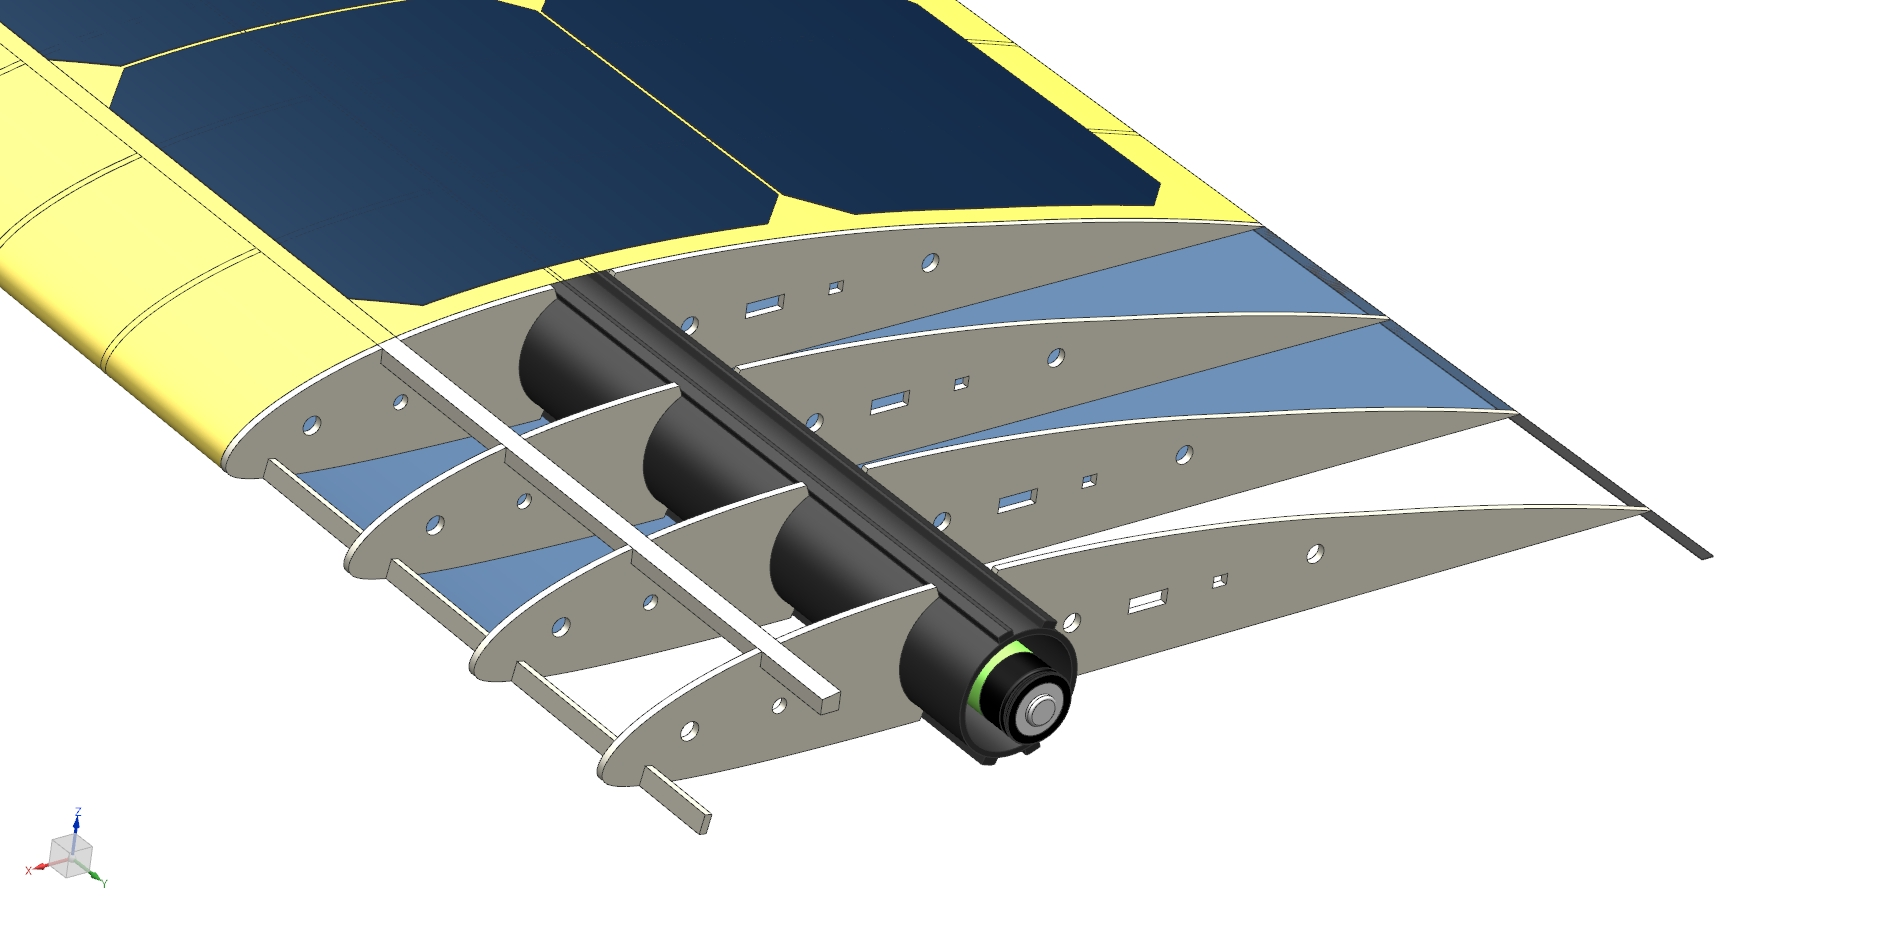
\includegraphics[width=\linewidth]{images/7_CAD_AtlantikSolarStructure}
    \caption{AtlantikSolar's wing structure, integrated batteries and solar cells.}
    \label{fig:CAD_AtlantikSolarStructure}
\end{figure}

The cylindrical wing spar contains a total of 60 cylindrical Lithium-Ion battery cells to optimally distribute the battery mass in a ``span loader'' concept. An additional 12 batteries can be added inside the outer wings to optimize the aircraft for a specific application. The Li-Ion cells are Panasonic NCR18650b high energy density (243Wh/kg) industrial cells.They are connected in a 6S (22.2V) configuration and provide $E_{bat,max}=850Wh$ at $m_{bat}=3.5kg$. The solar modules are seamlessly embedded into the upper wing surface to avoid premature flow separation. They feature a total of 88 SunPower C60 cells with a measured module-level efficiency of $\eta_{sm}=0.20$, an areal density of $k_{sm}=590g/m^2$ and a maximum power output of 275W at $\varphi=45°$ on June21\textsuperscript{st}. Modules featuring SunPower E60 cells with a verified module-level efficiency of $eta_sm=0.23$ are currently being integrated.

The propulsion system features a foldable carbon-fibre propeller with $D=66cm$ and 60cm pitch that was specifically developed to achieve $\eta_{propeller}=82\%$ at the nominal operating point of $F_{propeller}=2.4N$ at $v=8.5\unitfrac{m}{s}$. The propeller is driven by a 5:1 reduction-ratio planetary gearbox, a RS-E Strecker 260.20 brushless DC motor with $k_V=570RPM/V$ and a Kontronik Koby 55 LV motor controller. The propulsion system delivers a maximum electrical power of $P_{prop,max}=450W$. The actuation system consists of four Volz DA-15N servos that drive the two ailerons, the all-moving elevator and the rudder. To guarantee reliable multi-day flight, the Volz actuators were successfully bench-tested throughout a simulated continuous 30-day flight \cite{DellaCa_BT}.
%mention wind tunnel, lab motor test stand tests? Only if space left...

\subsubsection{Avionics}

The AtlantikSolar avionics topology is shown in Fig. \ref{fig:AtlantikSolar_SystemOverview} and an integration snapshot is presented in Fig. \ref{fig:9_CAD_AtlantikSolarAvionics}. Multiple sensors are centered around a Pixhawk PX4 Autopilot - an open source and open hardware project initiated at ETH Zurich - with a Cortex M4F microprocessor running at 168Mhz and featuring 192kB RAM. For state estimation (section XXX), an ADIS 16448 10-axis Inertial Measurement Unit (IMU), a u-Blox LEA-6H GPS receiver, and a Sensirion SDP600 differential pressure (i.e. airspeed) sensor are used. The SDP600 airspeed sensor has been chosen due to its low relative error of less than 5\% at airspeeds of 8m/s, which is necessary to closely control the airspeed to the airspeed with minimum required power $P_{out}$. Commands are received through a 433Mhz telemetry link for medium ranges, or through a long-range IRIDIUM-based satellite communication link that also serves as a backup in case of primary telemetry link failure. The airplane implements a fully manual RC-command fallback mode in case of a severe autopilot failure. Night operations are possible due to four on-board high-power LEDs.

\begin{figure}[tb]
    \centering
   % 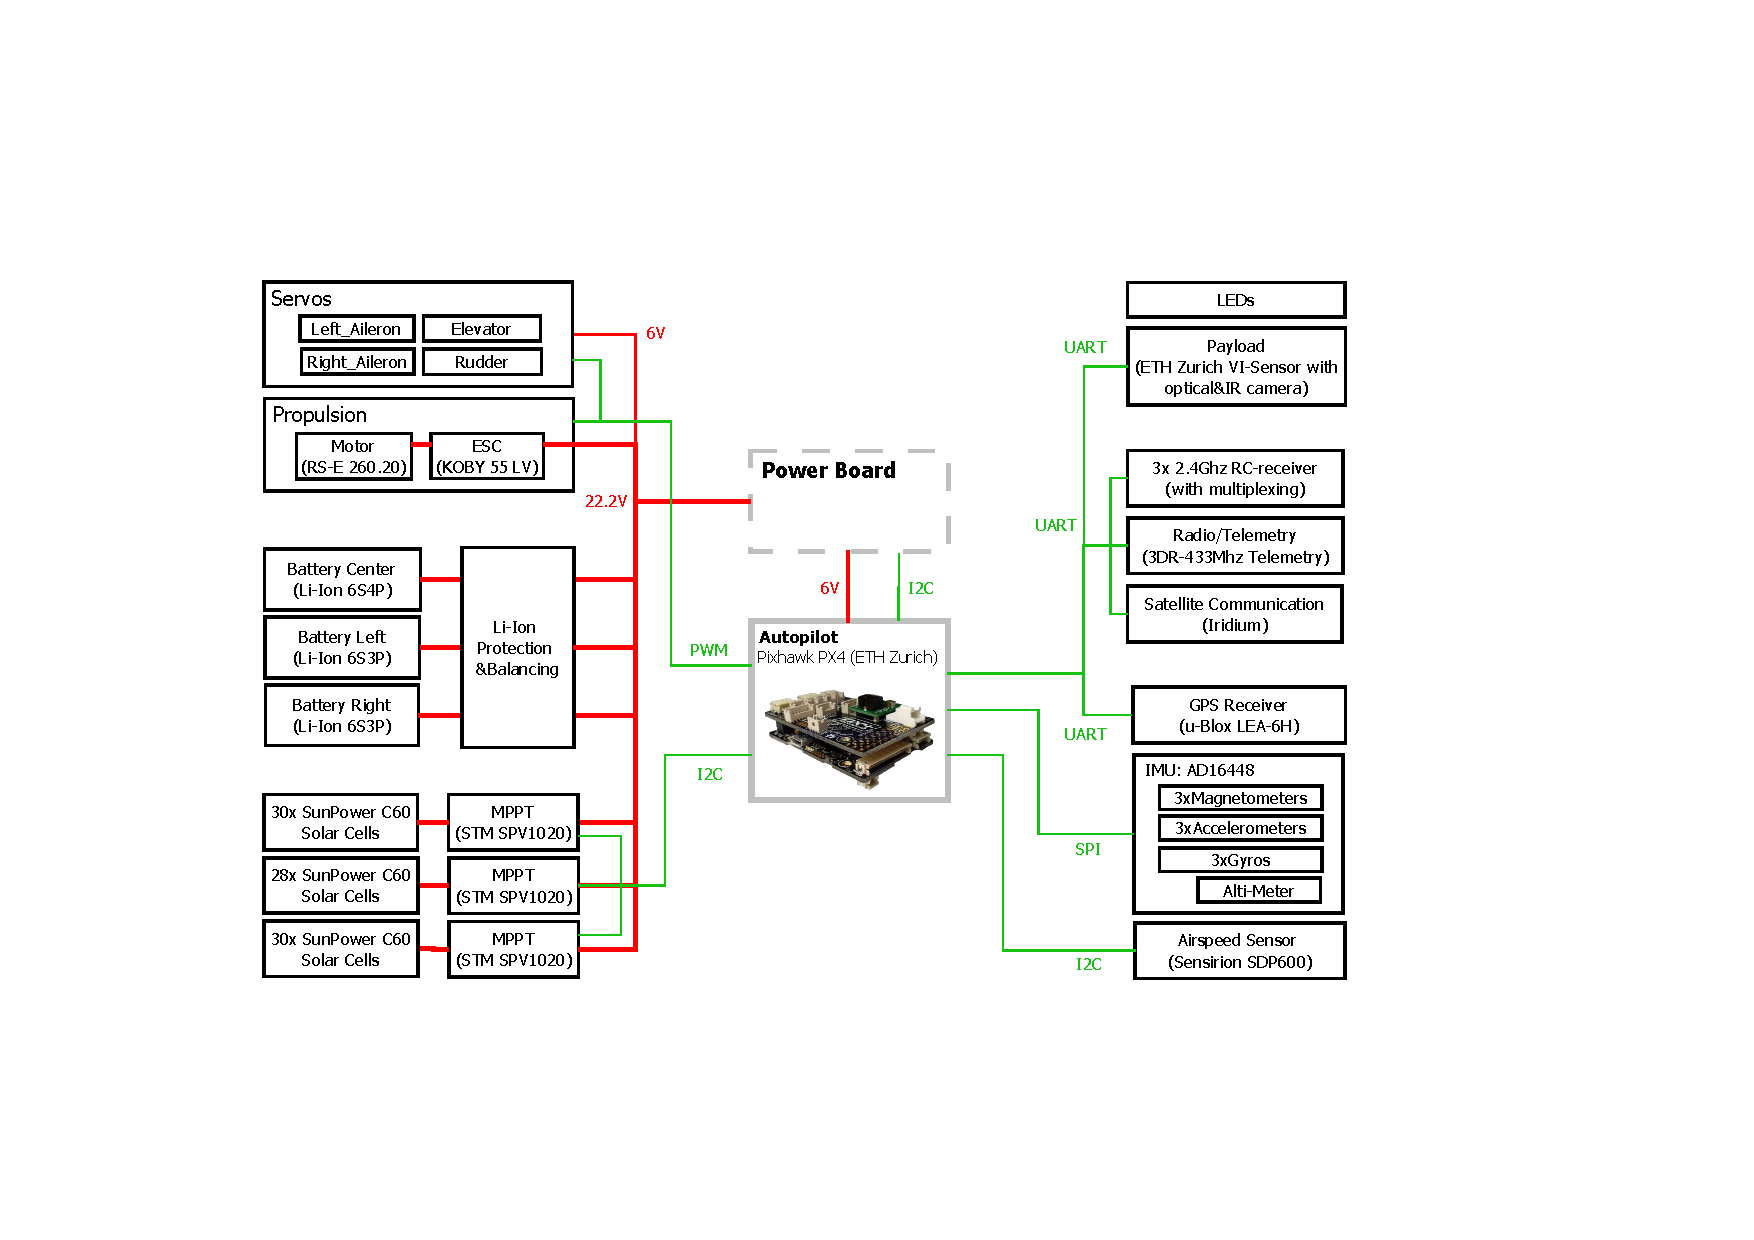
\includegraphics[width=\linewidth]{images/8_AtlantikSolar_Avionics}
     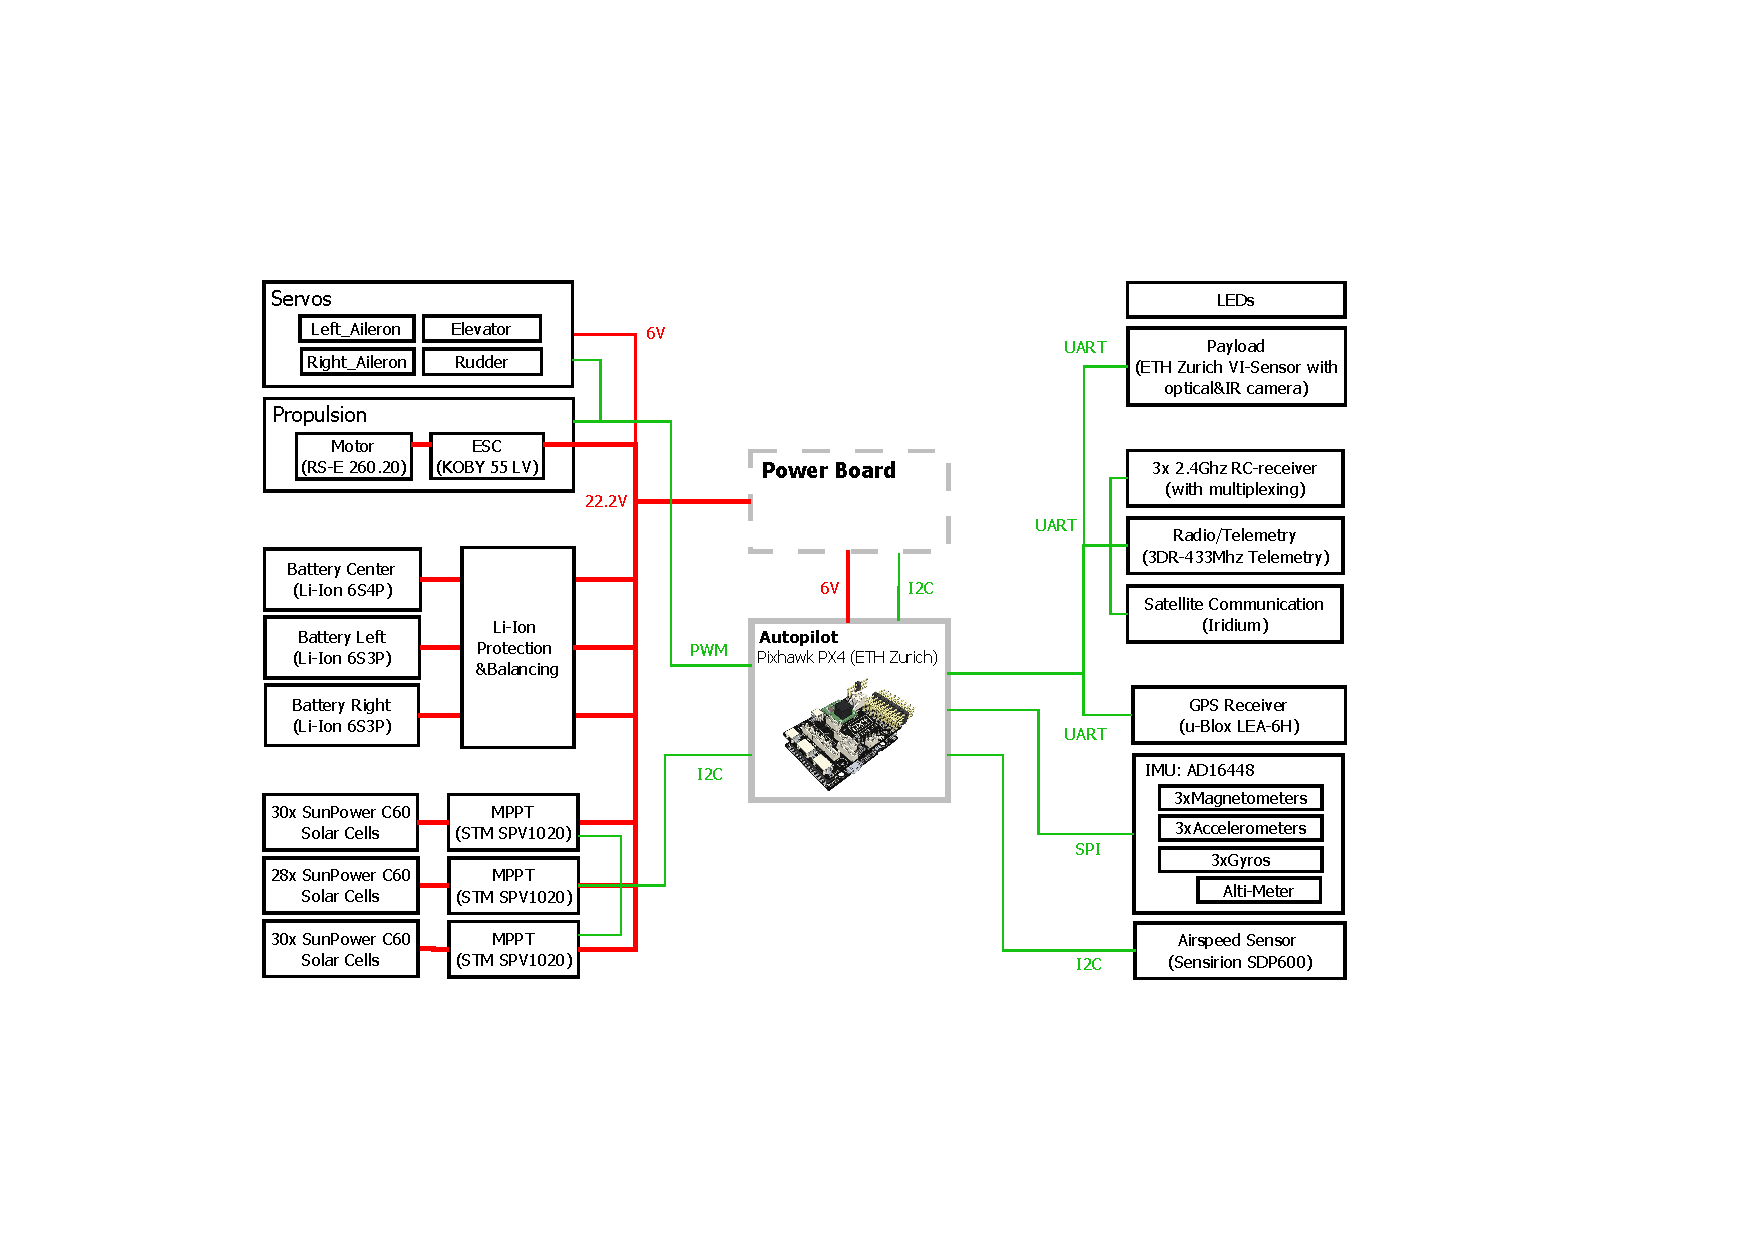
\includegraphics[width=\linewidth]{images/8b_AtlantikSolar_Avionics}
    \caption{AtlantikSolar system overview. For clarity, voltage lines from the autopilot to connected devices (5.0V and 3.3V) are omitted.}
    \label{fig:AtlantikSolar_SystemOverview}
\end{figure}

\begin{figure}[tb]
    \centering
    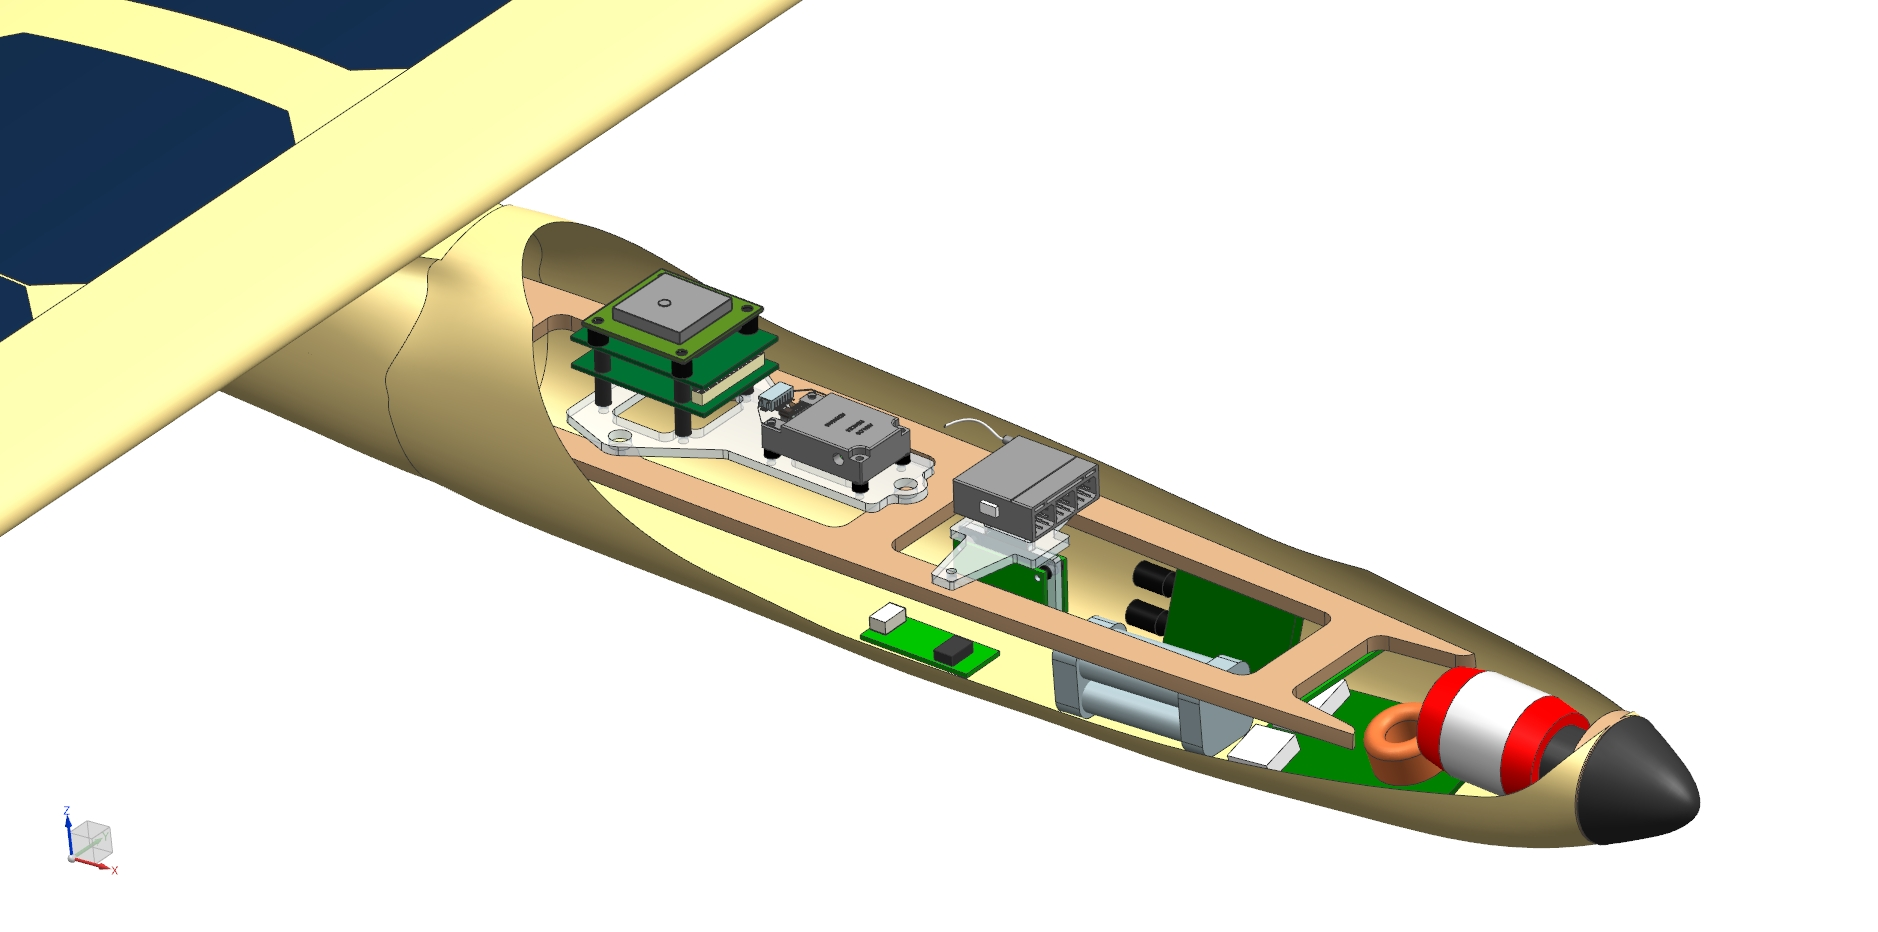
\includegraphics[width=\linewidth]{images/9_CAD_AtlantikSolarAvionics}
    \caption{Avionics components and their placement inside AtlantikSolar.}
    \label{fig:9_CAD_AtlantikSolarAvionics}
\end{figure}

\subsubsection{Payload}
% [THOMAS]
  - VI Sensor [ref to VI-sensor paper; ref to Leutenegger thesis?]
  - ~5 sentences + 1 picture
  
\subsection{State Estimation and Control Design}
%%%%%%%Onboard state estimation \& control					% why duplicate title?
\subsubsection{State estimation}
% [AMIR]
% - brief (5 sentence) description of SE type/principle
%  - one verification plot (e.g. gps position ``ground truth'' vs. estimated position) 
%  then REF to stefan\&Amir paper
The on-board state estimator based on extended Kalman filter (EKF) offers a robust estimation solution and can cope with prolonged GPS outage scenarios. It is implemented and optimized in order to grant full functionality on the on-board computation unit. 
Successive estimations of the position, velocity, orientation (attitude and heading), QFF, gyroscopes biases, accelerometers biases and the wind vector are rendered by the state estimator. Moreover additional estimations as the sideslip angle and the angle of attack (AoA) can be derived. A set of on-board sensors as inertial measurement unit (MEMS based), dynamic and static pressure sensors, magnetic compass and GPS receiver deliver the necessary data for the state estimator.A detailed description of the state estimator can be found in  \cite{Leutenegger_MSC2014}.

\begin{figure}[tb]
    \centering
    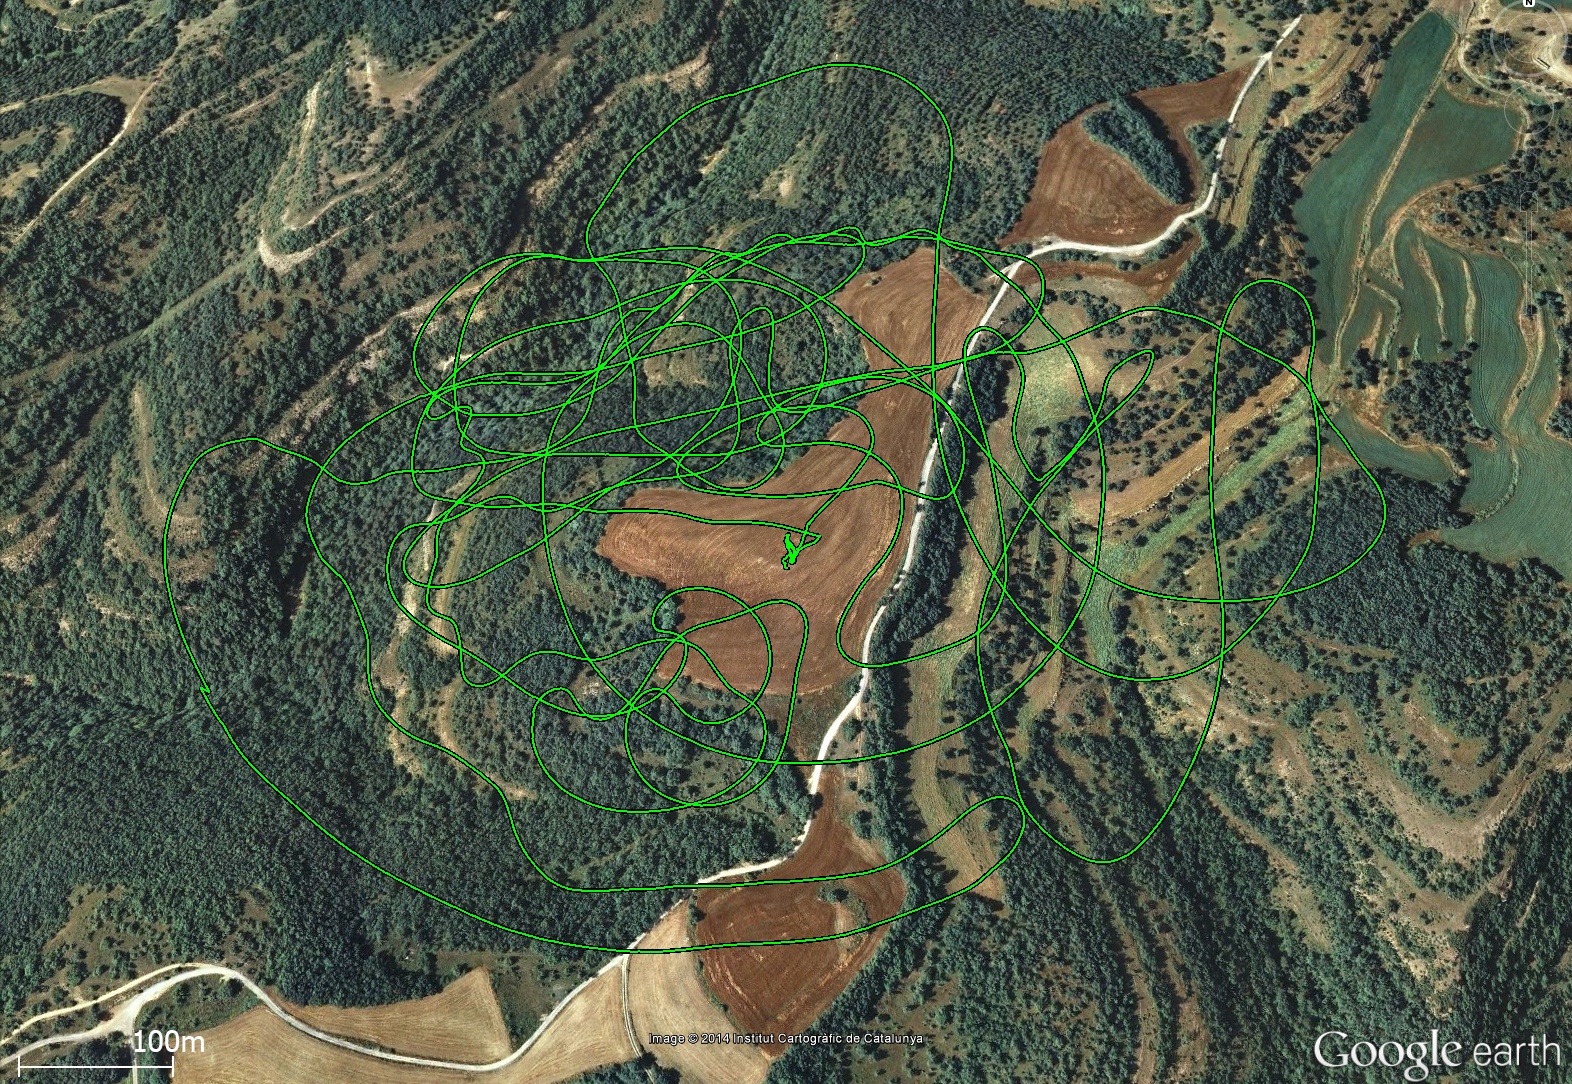
\includegraphics[width=\linewidth]{images/10_real_time_state_estimator_position}
    \caption{Overhead trajectories plot of the on-board position state estimation (green) and the GPS  (black).}
    \label{fig:real_time_state_estimator_positionl}
\end{figure}


\subsubsection{System Identification}
%[DR. ALEXIS]
 - System Identification \& Modelling
 
 \subsubsection{Control}
 %[PHILIPP writes this, DR. ALEXIS checks this]
 - Control using PID,  outer loops TECS \& L1 (Ref to OMLAS MED paper, also saying that there is future technologies which are being developed).
 - Full pre-flight verification in HIL
 
\subsection{Preliminary Results}
%[PHILIPP]
%if not in the sections before
  - control:   - SE\&Control: PID performance over various trim points. PID computational requirements (low!)
  - state estimation
  - solar system functioning
   - power efficiency curves. P\_level from Test flights.
   - potentially comparison to conceptual design 
   	- power (why not optimal: e.g. because optimal CD/CL\^1.5 assumed, but this has a) to be met in average and b) even then fluctuations as seen in flight tests are on the order of 2-3 degrees in AOA or +/- 1m/s, so this will never be met perfectly.
   	- actual mass vs. mass models?


%%%%%%%%%%%%%%%%%%%%%%%%%%%%%%%%%%%%%%%%%%%%%%%%%%%%%%%%%%%%%%%%%%%%%%%%%%%%%%%
% SECTION4: EXPERIMENTAL RESULTS
%%%%%%%%%%%%%%%%%%%%%%%%%%%%%%%%%%%%%%%%%%%%%%%%%%%%%%%%%%%%%%%%%%%%%%%%%%%%%%%
%%%%%%%%%%%%%%%%%%%%%%%%%%%%%%%%%%%%%%%%%%%%%%%%%%%%%%%%%%%%%%%%%%%%%%%%%%%%%%%
\section{EXPERIMENTAL RESULTS}
%%%%%%%%%%%%%%%%%%%%%%%%%%%%%%%%%%%%%%%%%%%%%%%%%%%%%%%%%%%%%%%%%%%%%%%%%%%%%%%
   
%PHILIPP]
 - mention total flight hours, total flights. Mention that 2 AtlantikSolars have already been built \& flown.  Range of weather conditions?
 
%%%%%%%%%%%%%%%%%%%%%%%%%%%%%%%%%%%%%%%%%%%%%%%%%%%%%%%%%%%%%%%%%%%%%%%%%%%%%%%
\subsection{Subsystem level results}
%%%%%%%%%%%%%%%%%%%%%%%%%%%%%%%%%%%%%%%%%%%%%%%%%%%%%%%%%%%%%%%%%%%%%%%%%%%%%%%
 
%[PHILIPP]. If not already done in the sections before.
   - power efficiency curves. P\_level from Test flights. Comparison to conceptual design. Describe why power consumption not optimal: e.g. because optimal CD/CL\^1.5 assumed, but this has a) to be met in average and b) even then fluctuations as seen in flight tests are on the order of 2-3 degrees in AOA or +/- 1m/s, so this will never be met perfectly.
 - solar system operation and recharge of batteries
 - state estimation (if not shown before)
 - control (if not shown before):   - SE\&Control: PID performance over various trim points. PID computational requirements (low!)
  
%%%%%%%%%%%%%%%%%%%%%%%%%%%%%%%%%%%%%%%%%%%%%%%%%%%%%%%%%%%%%%%%%%%%%%%%%%%%%%%
\subsection{Continuous 12hour Flight}
%%%%%%%%%%%%%%%%%%%%%%%%%%%%%%%%%%%%%%%%%%%%%%%%%%%%%%%%%%%%%%%%%%%%%%%%%%%%%%%
  
%[PHILIPP]
   - focus on battery performance. Say that even more possible (mention some results from the lab tests)
   - explain how much autonomous, under which conditions.
  
%%%%%%%%%%%%%%%%%%%%%%%%%%%%%%%%%%%%%%%%%%%%%%%%%%%%%%%%%%%%%%%%%%%%%%%%%%%%%%%
\subsection{Mapping Flights in Search and Rescue scenarios}
%%%%%%%%%%%%%%%%%%%%%%%%%%%%%%%%%%%%%%%%%%%%%%%%%%%%%%%%%%%%%%%%%%%%%%%%%%%%%%%
   
%[DRALEXIS]
    - mapping missions in ICARUS. 
    - REF to Separate paper??? Yes, but only once both are accepted.
    - some cool pics/reconstructed maps

%%%%%%%%%%%%%%%%%%%%%%%%%%%%%%%%%%%%%%%%%%%%%%%%%%%%%%%%%%%%%%%%%%%%%%%%%%%%%%%
\section{CONCLUSIONS}
 %%%%%%%%%%%%%%%%%%%%%%%%%%%%%%%%%%%%%%%%%%%%%%%%%%%%%%%%%%%%%%%%%%%%%%%%%%%%%%%
This paper presented the design, realization and flight testing of a solar-powered hand-launchable LALE UAV for robust (with respect to meteorological disturbances such as clouds) multi-day flight at 45\degree N geographical latitude from April 21\textsuperscript{st} to August 21\textsuperscript{st}. In-flight power measurements and a 12h 22min flight solely on batteries confirm the expected endurance and hence that flights through the night are possible. Achieving these performance results became possible through the thorough application of the presented extended conceptual design methodology along with significant engineering effort especially with respect to improving flight efficiency. Based upon the developed UAV platform, the next steps are to demonstrate one and multiple day-night (24h/48h) flights. Next to long-endurance research, more effort will be put into implementing advanced online localization, map reconstruction and planning capabilities into the existing optical and infrared camera pod to increase the autonomy in the SAR projects that the platform is involved in.

\addtolength{\textheight}{-12cm}   % This command serves to balance the column lengths
                                  % on the last page of the document manually. It shortens
                                  % the textheight of the last page by a suitable amount.
                                  % This command does not take effect until the next page
                                  % so it should come on the page before the last. Make
                                  % sure that you do not shorten the textheight too much.

%%%%%%%%%%%%%%%%%%%%%%%%%%%%%%%%%%%%%%%%%%%%%%%%%%%%%%%%%%%%%%%%%%%%%%%%%%%%%%%%

%%%%%%%%%%%%%%%%%%%%%%%%%%%%%%%%%%%%%%%%%%%%%%%%%%%%%%%%%%%%%%%%%%%%%%%%%%%%%%%%

\bibliographystyle{IEEEtran}
\bibliography{refs/refs_SolarUAVs,refs/refs_PhilippOePapers,refs/refs_AllOthers,refs/refs_KA}

\end{document}
